%%%%%%%%%%%%%%%%%%%%%%%%%%%%%%%%%%%%%%%%%
% Simple Sectioned Essay Template
% LaTeX Template
%
% This template has been downloaded from:
% http://www.latextemplates.com
%
% Note:
% The \lipsum[#] commands throughout this template generate dummy text
% to fill the template out. These commands should all be removed when 
% writing essay content.
%
%%%%%%%%%%%%%%%%%%%%%%%%%%%%%%%%%%%%%%%%%

%----------------------------------------------------------------------------------------
%	PACKAGES AND OTHER DOCUMENT CONFIGURATIONS
%----------------------------------------------------------------------------------------

\documentclass[12pt]{article} % Default font size is 12pt, it can be changed here

\usepackage{geometry} % Required to change the page size to A4
\geometry{a4paper} % Set the page size to be A4 as opposed to the default US Letter

\usepackage{graphicx} % Required for including pictures

\usepackage{float} % Allows putting an [H] in \begin{figure} to specify the exact location of the figure
\usepackage{wrapfig} % Allows in-line images such as the example fish picture

\usepackage{lipsum} % Used for inserting dummy 'Lorem ipsum' text into the template

\usepackage{hyperref}
\usepackage{color}

%\setlength\parindent{0pt} % Uncomment to remove all indentation from paragraphs

\graphicspath{{img/}} % Specifies the directory where pictures are stored

\begin{document}

%----------------------------------------------------------------------------------------
%	TITLE PAGE
%----------------------------------------------------------------------------------------

\begin{titlepage}

\newcommand{\HRule}{\rule{\linewidth}{0.5mm}} % Defines a new command for the horizontal lines, change thickness here

\center % Center everything on the page

\textsc{\LARGE Usability Engineering}\\[1.5cm] % Name of your university/college
\textsc{\Large CS/ISE 5714 - Spring 14}\\[0.5cm] % Major heading such as course name
\textsc{\large  Project 2: Contextual inquiry and contextual analysis}\\[0.5cm] % Minor heading such as course title

\HRule \\[0.4cm]
{ \huge \bfseries The Writing Center }\\[0.4cm] % Title of your document
\HRule \\[0.4cm]
{ \small Inkhorn: a scheduling and feedback system to help tailor coaching services to patrons }\\[0.4cm] % Title of your document
\vspace{1.5cm}


\begin{minipage}{0.4\textwidth}
\begin{flushleft} \large
\emph{TEAM 1:}\\
TC \textsc{Jones} \href{mailto:tjones21@vt.edu}{\textcolor{blue}{tjones21@vt.edu}}\\
Rebecca \textsc{Zeitz} \href{mailto:razeitz@cs.vt.edu}{\textcolor{blue}{razeitz@vt.edu}}\\
Chris \textsc{Frisina}  \href{mailto:special@vt.edu}{\textcolor{blue}{special@vt.edu}}\\
\end{flushleft}
\end{minipage}
~
\begin{minipage}{0.4\textwidth}
\begin{flushright} \large
\emph{Client:} \\
Jennifer \textsc{Lawrence}  \href{mailto:jlwrnc@vt.edu}{\textcolor{blue}{jlwrnc@vt.edu}}\\
\end{flushright}
\end{minipage}\\[4cm]

{\large \today}\\[3cm] % Date, change the \today to a set date if you want to be precise

%\includegraphics{Logo}\\[1cm] % Include a department/university logo - this will require the graphicx package

\vfill % Fill the rest of the page with whitespace

\end{titlepage}

%----------------------------------------------------------------------------------------
%	TABLE OF CONTENTS
%----------------------------------------------------------------------------------------

\tableofcontents % Include a table of contents
\newpage % Begins the essay on a new page instead of on the same page as the table of contents 

%----------------------------------------------------------------------------------------
%	INTRODUCTION
%----------------------------------------------------------------------------------------

\section{Concept Statement} % Major section

% What is the system name?  
% –Who are the system users?  
% –What will the system do? 
% –What problem(s) will the system solve? (Be broad to include business objectives)
% What is design vision and what are the emotional impact goals?
% what experience will system provide to user
% Audience broader than that of most other deliverables, including   
% – High-level management 
% – Marketing 
% – Board of directors  
% – Stockholders  
% – Even general public

% Rebecca
% Inkhorn will serve the Writing Center by providing a common ground tool for use among coaches and other staff.  It will allow users, the Writing Center staff, to match coaches with patrons requesting a session by providing a more systematic, but still personalized, scheduling process.  As a feedback system, Inkhorn will allow for patron privacy not currently available.  Furthermore, Inkhorn will serve as a tool for coaches to suggest resources and methods that will coincide with the needs and goals of the patrons.  Inkhorn will help tailor writing enhancing coaching services to specific patrons’ needs, such as with conference or course papers, technical documents, personal statements, or other interpersonal communications.  Playing off the informal but professional atmosphere of the Writing Center, Inkhorn will be a space for users to converse and share thoughts and ideas.  In essence, Inkhorn will act as a bridge between the coaches, administrative staff, and patrons.

The Virginia New River Valley community members often seek support services surrounding improving their communication skills and understanding of the English language.
The Virginia Tech Writing Center (WC) provides varying personal coaching services for these locals in addition to VT affiliates.
Inkhorn, an automated scheduling and feedback system, will help tailor coaching services to patrons to develop their skills to enhance their writing, such as conference or class papers, personal statements, and interpersonal communications. 
Inkhorn will help promote services offered by WC, manage session scheduling with compatible coaches, automate reporting, provide a continual coach feedback system, manage forms, and suggest appropriate tools for patron goals.

%------------------------------------------------

\section{Choosing a Client Process} % Sub-section

Among our initial ideas for clients and problems, we focused on writing.
Our initial problem was in the realm of collaborative writing techniques for technical, novel, and story telling writers.
Given client scheduling problems, we had to abandon this idea.
Our next client in the writing domain we chose was the Virginia Tech Writing Center (WC), and the Assistant Director Jennifer Lawrence.
She has served in this role for 7 years, and her extensive knowledge alongside positional status makes her the ideal candidate within the WC to initially contact and get organizational information, as well as follow communication for project details.

3 


\subsection{Description} % Sub-section

\subsection{Interviews} % Sub-section

4 | 5 | 6 | 7

\subsubsection{WADD} % Sub-sub-section

For building the Work Activity Affinity Diagram (WAAD), the raw data was synthesized into work activity notes, which were written on green and yellow sticky notes so that the colors would blend together.
We left the bolder colors for the hierarchical categorization labels for the developed clusters of notes.  Each work activity note was given a source ID.
The first part of the interview with Jennifer Lawrence concerning the work role of Assistant Director of the Writing Center was denoted by the source ID “ADIR”.
The second part of that interview that concerned her work role as a Writing Center coach was denoted by the source ID “C1”.
For the interview with Nneoma Enyi Nwankwo, a writing center coach, the source ID of “C2” was used. 

Our team added the sticky notes to a whiteboard, grouping similar activity notes together and rearranging them as new notes were added or new connections or relationships between the activity notes were recognized.  Once a category was formulated, top-level cluster labels, the blue sticky notes in the images, were added atop their respective clusters.  Some of these top-level cluster labels were representative of work roles.  If two notes were recognized as holding the same content, one note was stuck to the bottom of the other, so that they were grouped together.  This stage of the process is represented by the WAAD version 1 image. 

The top-level cluster labels were good for overall categorization, but the clusters from these were too broad.  These clusters were further broken down into sub-sections by grouping the activity notes into even more specific clusters, which indicated more specific, sub-level cluster labels, the orange sticky notes in the images.  In the WAAD version 2 image, this process of sub-clustering also resulted in the creation of a new top-level cluster label, Coach-Patron Interactions which pulled notes out of the Coach and Patron clusters.   The WAAD version 3 image shows the formalization of three of the top-level and 7 of the sub-level clusters.  The sub-level clustering process was repeated for the remaining clusters, as seen in the WAAD version 4 until the result was the final WAAD version 5.
% WADD PICTURES
\begin{figure}[H] % Example image
\center{
\includegraphics[width=0.5\linewidth]{placeholder}}
\caption{Example image.}
\label{fig:speciation}
\end{figure}

%------------------------------------------------

\section{Work Roles} % Sub-sub-section
  \begin{description} % Numbered list example
  \item[Director]
  Diana George
  \item[Assistant Director]
  Jennifer Lawrence (7 years in this position)\\
  The Assistant Director is in charge of hiring all coaches, scheduling coach work allotments, reports, a
  \item[Administrative Staff]
  Sandra Ross \\
  This role is in charge of making the consolidated reports and trends that are received from the Scheduler, and providing administrative assistance to the Director and Assistant Director. 
  \item[Graduate Assistant to the Director]
  Katharine Torrey \\
  This is a special coach that in addition to normal coach role duties, also helps with some of the tasks that are oriented towards the coaches, speaking as representative for the coaches and a supporting voice for the Assistant Director.
  \item[Coach] \hfill \\
  These are under/graduate students who have a strong skill set in the English language.
  They are required to have an application, strong GPA, a letter of recommendation from a VT faculty member , have passed the English 3744 class, and ideally a second language, double major, and/or honor student.
  \item[Patron] \hfill \\
  Any local resident of the New River Valley, with or without VT affiliation, who wants help improving their communication skills ()
  \item[VT Professor] \hfill \\
  A professor or lecturer at Virginia Tech.
  \item[Scheduler] \hfill \\
  A coach at the WC that is currently not seeing a patron, who makes appointments in the schedule book.
  \item[Paperwork Organizer] \hfill \\
  A coach at the WC that is currently not seeing a patron, who arranges the session paperwork to hand to the Admin person.
  \item[Funding] \hfill \\
  People or entities, predominately but not always affiliated with VT, that provide monetary funds to the WC for operational costs.
  \end{description} 
\section{Flow Diagram}



\section{Photos} % Major section

\subsection{Interviews} % Sub-section

\subsection{Raw Data Notes} % Sub-sub-section
  \subsubsection{Task Data Notes} % Sub-sub-section
  \subsubsection{Audio Interview Notes} % Sub-sub-section
  \href{http://www.dropbox.specialorange.com/vt/5714%20UX/}{\textcolor{blue}{Audio Folder}}\\
  \href{http://www.dropbox.specialorange.com/vt/5714%20UX/ADir1.aac}{\textcolor{blue}{Assistant Director 1}}\\
  \hspace{1.5cm}\href{http://www.dropbox.specialorange.com/vt/5714%20UX/C1.aac}{\textcolor{blue}{Coach 1}}\\

\subsection{Task Data} % Sub-sub-section

\subsection{Artifacts} % Sub-sub-section

text
\begin{figure} % Inline image example
  \begin{center}
    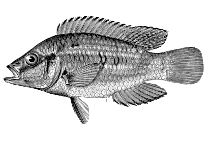
\includegraphics[width=0.38\textwidth]{fish}
  \end{center}
  \caption{Fish}
\end{figure}

%----------------------------------------------------------------------------------------
%	CONCLUSION
%----------------------------------------------------------------------------------------
\section{Conclusion} % Major section


%----------------------------------------------------------------------------------------
%	BIBLIOGRAPHY
%----------------------------------------------------------------------------------------
\begin{thebibliography}{99} % Bibliography - this is intentionally simple in this template

  \bibitem[Figueredo and Wolf, 2009]{Figueredo:2009dg}
  Figueredo, A.~J. and Wolf, P. S.~A. (2009).
  \newblock Assortative pairing and life history strategy - a cross-cultural
    study.
  \newblock {\em Human Nature}, 20:317--330.
 
\end{thebibliography}

\end{document}